\documentclass{llncs}

\usepackage{subcaption}
\usepackage{subfig} 
\usepackage{usual}
\usepackage{graphicx}
\usepackage[noend]{algpseudocode}
\usepackage{subcaption}
\usepackage{subfig} 
\pagestyle{plain}

%
\begin{document}
\title{Agent utterances in dialogue of cooperative negotiation}
\maketitle 
Explain that for each utterance chosen by the user, we designed a tree of all the possible responses. These responses take in account the principals of dominance that we aim to model and the current state of the negotiation.
\section{State Preference}

When the user states a preference. We note StatePreference(C, less,more), where $less, more \in C$. Figure 1; depicte the tree of choices, where each branch depends on the satisfiability of an applicability condition

\begin{itemize}
	\item \textbf{Propose(C,More):} The agent proposes the preferred value. The agent proposes a value only and only if the value is acceptable for the agent. However, the value of acceptability varies depending on the value of dominance. 
		\subitem The acceptability of a value is computed with a function that considers the relation of dominance. First, dominant agent is very demanding, while the submissive one is not. Second, the submissive considers the preferences of the user. Indeed, if the user proposes a value that the agent already stated as not preferred, the agent will avoid a conflicting situation and accepts the value. Therefore the function isAcceptable(value, relation) is defined as follow: 
		\begin{figure}[]
			\begin{algorithmic}[1]\small
				\Function{isAcceptable}{$value$, $relation$}
					
					\If{($relation = dominant$)} 
						\State return $(score(value)> bestScoreOfPreference \times 0.7)$
					\EndIf
					\If{($relation = peer$)} 
						\State return $(score(value)> 0)$
					\EndIf
					\If{($relation = sub$)} 
						\State return $(score(value)> 0$  or $isInOAS(value))$
					\EndIf
				\EndFunction
			\end{algorithmic}
			\vskip 8pt
			\defig{pseudo}{Function to compute the acceptability of a value of preference}
		\end{figure} 
		
	\item \textbf{StatePreferenc(C,less',more')} : the agent reacts to the stated preference expressed by the user
	
			\begin{figure}[h]
					\begin{algorithmic}[1]\small
						\Function{reactToUser}{$less$, $more$}
							
							\If{($more = MostPrefferedValue()$ and $ (*, more) \notin OAS$)} 
								\State return $(*, more)$
							\EndIf
							\If{($more = LeastPrefferedValue()$ and $ (more, *) \notin OAS$)} 
								\State return $(more, *) $
							\EndIf
							\State The conditions $(2,4)$ are also applied for $less$
							\State $(less',more') = computePreference(less,more)$
							\If {$(less',more') \in OAS$}
								\State $(less1,more1)= reactToCriterion(more)$
								\If {$(less1,more1)=null$}
									\State $(less2,more2)= reactToCriterion(less)$
										\If{ $(less2,more2)=null$}
											\State return $(less',more')$
											\Else  
												return $(less2,more2)$
										\EndIf
								\EndIf
							\EndIf
							\State return $(less', more')$
						\EndFunction
						\Function{reactToCriterion}{$criterion$}
						\EndFunction
					\end{algorithmic}
					\vskip 8pt
					\defig{pseudo}{Function to react to a preference (less,more)}
				\end{figure}
		
		\item \textbf{AskPreference(C,less, more)}:

		
		
\end{itemize}
%

\section{AskPreference: } 
		When the user asks the agent about a preference, the agent calls the function reactToUser to compute a preference.
		
\section{Propose(proposal)}
	the user can either propose a value for a criterion or an option from the set of options of the topic of conversation. Thus, we define a proposal as a tuple $Proposal(Type, Value)$ where  $Type$ is either the the topic (for example Restaurants) or a criterion $c \in \mathcal{C}$ and value is:
	\begin{itemize}
		\item an option $O \in \in \mathcal{O}$ if $Type \in Topic$ 
		\item a value $v \in \emph{D}_c$ if $Type \in \mathcal{C}$
	\end{itemize}
	   
\begin{itemize}
	\item In the case where a user proposes an option that is acceptable for the agent this later calls the task \textit{Booking}, to ask the user to book a table for the restaurant. 
	\item \textbf{Accept(Proposal):} the user proposes a value for a criterion that is acceptable for the agent. Thus, the agent expresses an accept.
	\item \textbf{Propose(Proposal'):} The user proposes a proposal which is not acceptable for the agent. This branch is applicable only if the agent is dominant in the relation. A dominant agent is demanding and self centered. Thus, if a user proposes a value which is not acceptable, the agent will counter propose with another value that better suits its preferences.
	\item \textbf{StatePreference(less,more):} The user proposes a proposal which is not acceptable for the agent, and the agent is submissive in its relation with the user. Instead of expressing a reject, the submissive agent will express a statement to express that the proposed value doesn't suit its preferences.
	In the case of an option, the agent computes the least scored value of this option to explain why he doesn't accept the proposal.
	\item\textbf{Reject(Proposal):} In the same case where the proposed value is not acceptable but the agent is not submissive to express his reject.
		
\end{itemize}

\section{Accept(proposal)}

\item \textbf{Booking: } When the user accepts an option proposal , the agent closes the negotiation by proposing to book a table for the accepted restaurant (option).

\item \textbf{Propose(ProposalO):} when a user accepts a criterion proposal, a non-submissive agent continues the negotiation and proposes an option that is defined with the accepted value. However, a submissive agent will only propose an option, if the user accepts a value for each criterion of the topic.  The proposed option is defined with all the accepted values.
\item after accepting a value for a criterion, the agent opens a negotiation about another criterion of the topic to keep going on the negotiation. Wi distinguish three different responses with respect to the relation of dominance with the user:

	\subitem \textbf{StatePreference(less,more)}:  A peer agent opens a new subtopic or a negotiation on a criterion by expressing his preferences on this criterion.
	\subitem \textbf{AskPreference(less,more)}:  A submissive agent considers the preferences of the user and aims to satisfy them. Thus, to open a new negotiation on a criterion, he asks the user about his preferences on this criterion.
	\subitem \textbf{Propose(Proposal):} a dominant agent only considers his preferences. Thus, he directs the negotiation to satisfy them, by proposing his most preferred value on the new criterion. 

\section{Reject(proposal)}

%\par In this document, I'll present the different cases of agent responses to a user utterance. 
%I'll first define the utterances arguments to make the document readable.
%\begin{itemize}
%\item Lets $x$ be a value of a criterion. Thus, we note for this document the fact of stating preference on $x$ means either $p(x,i)$ or $p(i,x)$, where $x \not=  y$  and $x, i \in \mathcal{D}_C$.
%\item We define the value $y$ such that  $x, y \in \mathcal{D}_C$.
%\item We define the value $z$ such that  $x\in \mathcal{D}_C$ and $z \notin \mathcal{D}_C$, which means that $x$ and $z$ represent the value of two different criteria.
%\item $O$ is an option.
%\end{itemize}
%
%\section{State Preference}
%In the dialogue, the user might state a preference on a value of a criterion named $X$. In this case, the agent can response with the utterances defined in the \fig{state}. 
%
%\begin{figure}[b]
%\centerline{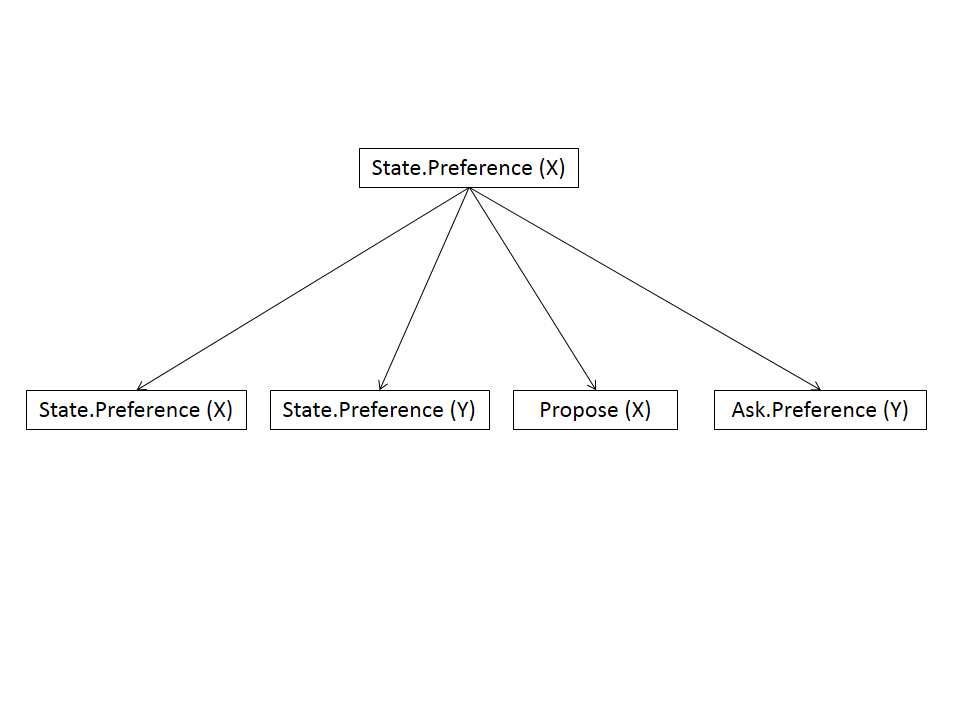
\includegraphics[width=5in]{figs/state.PNG}}
%
%\defig{state}{state preference response.}
%\end{figure}
%\begin{enumerate}
%\item State.Preference($x$): This is the most accurate response that I found in the example dialogue with lauriane and leonor. 
%For example, 
%\\ - leo: state.Preference(Breton, *).
%\\ - laur: State.Preference(*,Breton).
%
%\item State.Preference($y$): the agent can answer with its preferred value for the same criterion. For example,
%\\ - User: I like the most japanese cuisine.
%\\ - Agent: I like the most indian cuisine.
%
%\item Propose (X): We can imagine that the agent prioritize the user preferences. Thus, is the user prefers $x$ the agent would propose it.
%For example:
%\\- User : I like the V arrondissement.
%\\- Agent: Lets choose the V arrondissement. 
%
%\item Ask.Preference(Y): The agent cas ask the user to give more information about its preferences.
%\\ - User: I like the most japanese cuisine.
%\\ - Agent: Do you like indian cuisine? 
%\end{enumerate}
%
%
%
%\section{Ask Preference}
%\begin{figure} [t]
%	\centerline{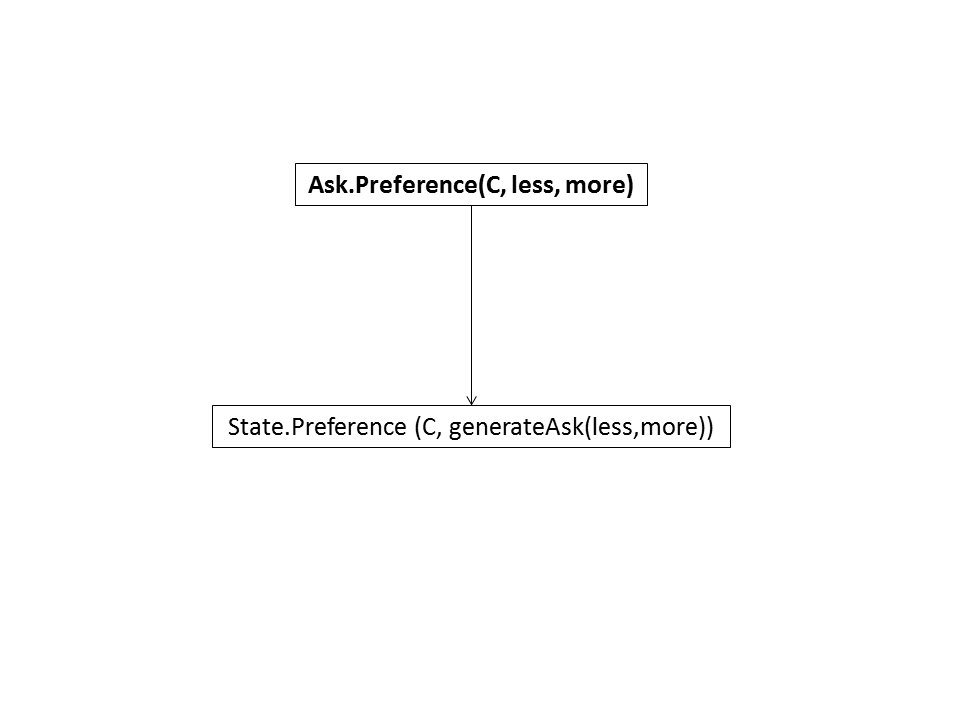
\includegraphics[width=5in]{utterances/Diapositive1.PNG}}
%	\vskip 8pt
%	\defig{ask}{agent possible answers to an ask Preference}
%\end{figure}
%\begin{figure}
%\centerline{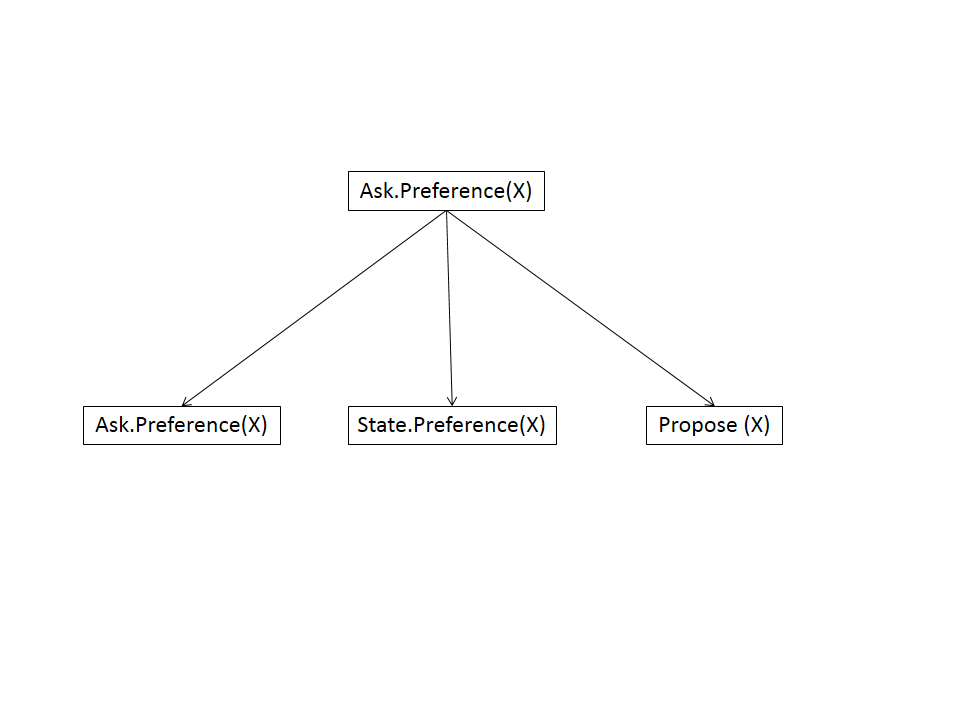
\includegraphics[width=5in]{figs/ask.PNG}}
%
%\defig{ask}{ask preference response.}
%\end{figure}
%
%When the agent receive an ask.Preference utterance, it can use the following utterances which are illustrated in \fig{ask}.
% \begin{enumerate}
% \item State.Preference($x$): This is the most logical response is to response with the agent preferences on $x$. In the dialogue with lauriane and leonor, I found this example:  
% \\ - leo: Ask.Preference(Italian).
% \\ - laur: State.Preference(Italian, *). 
% 
%% \item Propose(X): In the same idea that the agent prioritize the user preferences. Thus, is the user prefers $x$ the agent would propose it. 
%% For example:
%% \\- User : I like the V arrondissement.
%% \\- Agent: Lets choose the V arrondissement. 
%% \\ However, this utterance is not applicable in the case where the user asks for a criterion( example: which type of cuisine do you like ?).
%% 
% \item Ask.Preference(Y): Assuming that the agent is very submissive, he can prefer ask for the user preference on $x$ rather than expressing its preference.
% \\ - User: Do you like indian cuisine ?.
% \\ - Agent: Do you like indian cuisine? 
% \end{enumerate}
%
%\section{Propose}
%I distinguish here when the propose has as attribute a $x$ or an option $O$. 
%Take first the case where an option is proposed and, I assume that $V(O,C) = x$.
%
%\begin{figure}
%\centerline{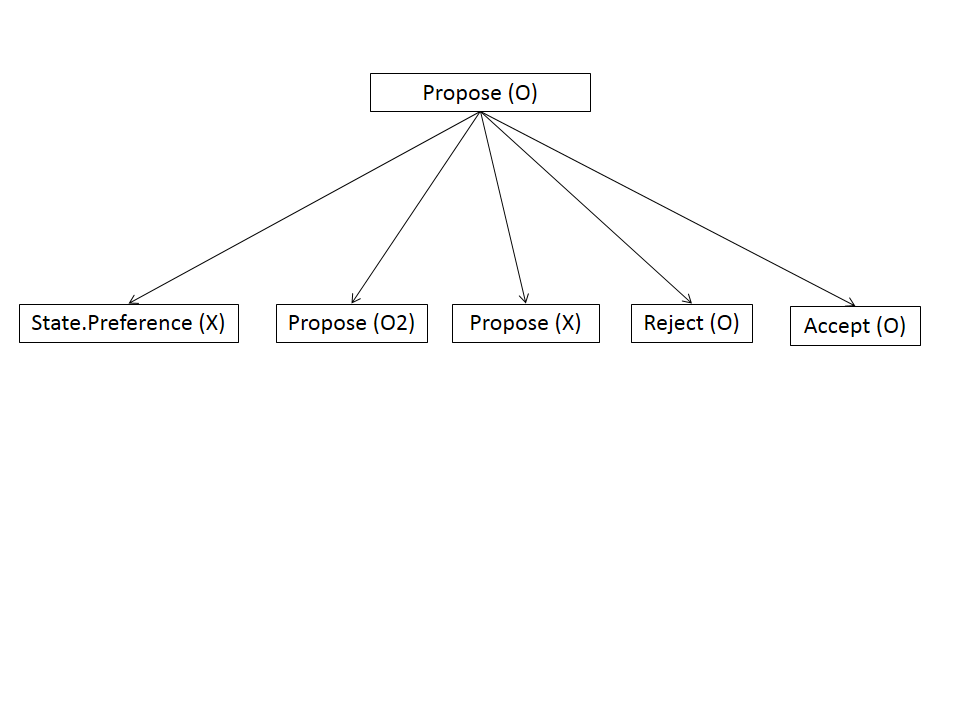
\includegraphics[width=5in]{figs/proposeO.PNG}}
%
%\defig{propO}{agent possible answers to a proposing an option}
%\end{figure}
%
%\begin{enumerate}
%\item Reject(O): The agent can reject the proposal.
%\\ - leo: Propose(africain).
%\\ - laur: Reject (africain). 
%\item Accept(O): The agent can accept a proposal.
%\\ - leo: Propose(africain).
%\\ - lau: Accept(africain). 
%\\ In this example of lauriane and leonor dialogue, we can notice that lauriane accepts africain  knowing that she rejected this proposal earlier in the dialogue. This is can be explained by the fact that leonor used arguments to convince lauriane to like africain, and lauriane clearly said it \textit{"Mais africain  me tente bien, tu m'as bien vendu le truc"}. For the moment, we are not able to express argumentation. 
%
%\item Propose (X):the agent can counter propose with only a value of a criterion $x$. 
%For example:
%\\ User: Lets go to Ginza restaurant
%\\ Agent: Lets go to a french restaurant. 
%
%\item Stat.ePreference($x$): We can assume that the agent is not dominant enough to feel at his  ease to express a reject. Therefore, he expresses its preference on the value that he doesn't like. For example
%\\ User: Lets go to Ginza restaurant
%\\ Agent: I don't like chinese cuisine.  
%\end{enumerate}
%
%\begin{figure}
%\centerline{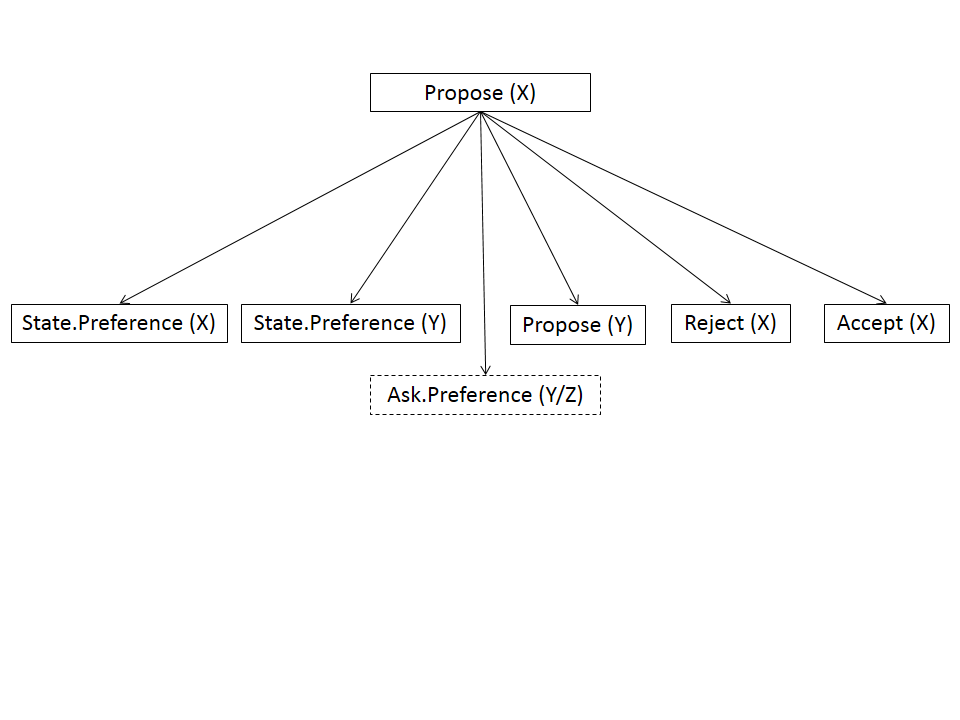
\includegraphics[width=5in]{figs/proposeX.PNG}}
%
%\defig{propx}{agent possible answers to a propose value}
%\end{figure}
%\par The agent responses to a value are very similar to the option. I separate them to be easer to explain. 
%\begin{enumerate}
%\item Reject(X): The agent can reject the proposal.
%\\ - User: Propose(japanese).
%\\ - agent: Reject (japanese). 
%\item Accept(O): The agent can accept a proposal.
%\\ - User: Propose(cheap).
%\\ - Agent: Accept(cheap). 
%
%\item Propose (y):the agent  counter propose with another value $y$. 
%For example:
%\\ - User: Propose(japanese).
%\\ - agent: Propose (italian). 
%
%\item propose(O): the agent can counter propose with an option, like in the dialogue example where lauriane counter proposed leonor proposal with a restaurant proposal. 
%\\ - leo: Propose(Aveyronnais)
%\\ -laur: propose(CheeseClub)
%
%
%\item State.Preference($x$/$y$): We can assume that the agent is not dominant enough to feel at his  ease to express a reject or an counter proposal. Therefore, he expresses its preference on the value that he doesn't like to invite the user to reject this value, or to state his preference for something that he likes to invite the user to propose it. For example
%\\ User: Lets go to a chinese restaurant
%\\ Agent: I don't like chinese cuisine.
%\\ Or
%\\ agent: I really like french cuisine. 
%
%\item Ask.Preference(y):  Debate wether model an ask here or not. I think that we don't have to keep it.
%\end{enumerate}
%
%
%\section{Accept}
%
%\begin{figure}
%\centerline{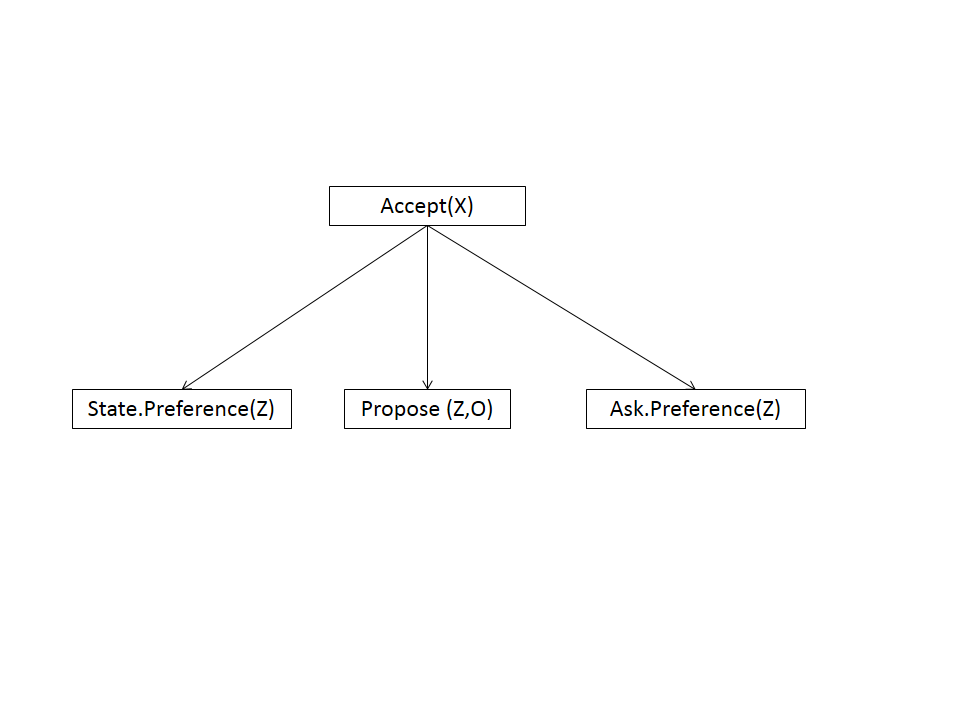
\includegraphics[width=5in]{figs/accept.PNG}}
%\defig{accept}{Accept utterance}
%\end{figure}
%
%If the user make an accept for an option $O$. It will close the dialogue because the main goal is satisfied. Whereas, accepting a value for a criterion may open the dialogue for the resting of the criteria or options. 
%\begin{enumerate}
%\item propose(O/Z): the agent can either propose an option where $v(O,C) =x$ or propose a value for another criterion.
%\\ - User: Accept(Aveyronnais)
%\\ - Agent: propose(SAVEURS D'AVEYRON )
%\\Or
%\\ Agent: propose(cheap)
%
%
%\item the agent can move to the negotiation on other criteria. Thus, it can express his preferences or ask the user preferences on theses criteria. 
%
%\item State.Preference($z$) for example
%\\ User: Accept(Aveyronnais)
%\\ Agent: State.Preference(calm, noisy): I prefer calm ambiance more than noisy ambiance.
%
%
%\item Ask.Preference($z$): For example
%\\ User: Accept(Aveyronnais)
%\\ Agent: ask.Preference(calm) : do you like calm ambiance?
%\end{enumerate}
%
%\section{Reject}
%
%\subsection{Reject an option}
%
%\begin{figure}
%\centerline{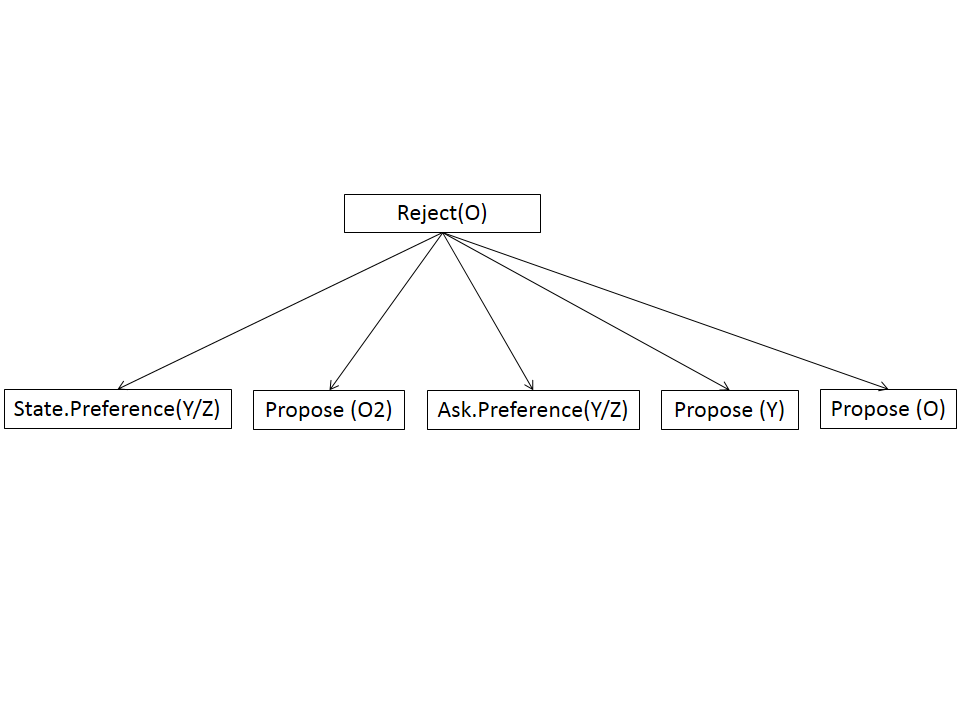
\includegraphics[width=5in]{figs/rejectO.PNG}}
%\vskip 8pt
%\defig{rejO}{agent possible answers to reject a an option}
%\end{figure}
%
%\par When the user reject an option, I thought that it might be interesting to add an utterance yo ask him why rejected this option. I think to a simple utterance where the user can tell us for example that he doesn't like the cuisine or the ambiance of this restaurant. 
%
%\begin{enumerate}
% 
%\item propose($O_2$): the agent can  propose another value to the user. For example
%\\ - User: Reject(cheeseClub): No, I'd raher choose another restaurant.
%\\ -Agent: propose(chez chuck): Let's choose chez chuck!
%
%\item propose($O$): the agent can  propose the same restaurant again because he's very dominant
%\\ \textbf{warning}: Loop, we have to stop the agent to make the same proposal several times.
%
%
%\item Propose (y):the agent  can also propose another value $y$. 
%For example:
%\\ - User: Reject(cheeseClub). where (v(cheeseClub, cuisine) = fromage)
%\\ - agent: Propose (italian). 
%
%\item State.Preference($z$/$y$): the agent can state its preferences on other values for the different criteria. For example
%\\ User: Reject(cheeseClub)
%\\ agent: I like the most french cuisine. 
%
%\end{enumerate}
%
%\subsection{Reject a value}
%\begin{figure}
%\centerline{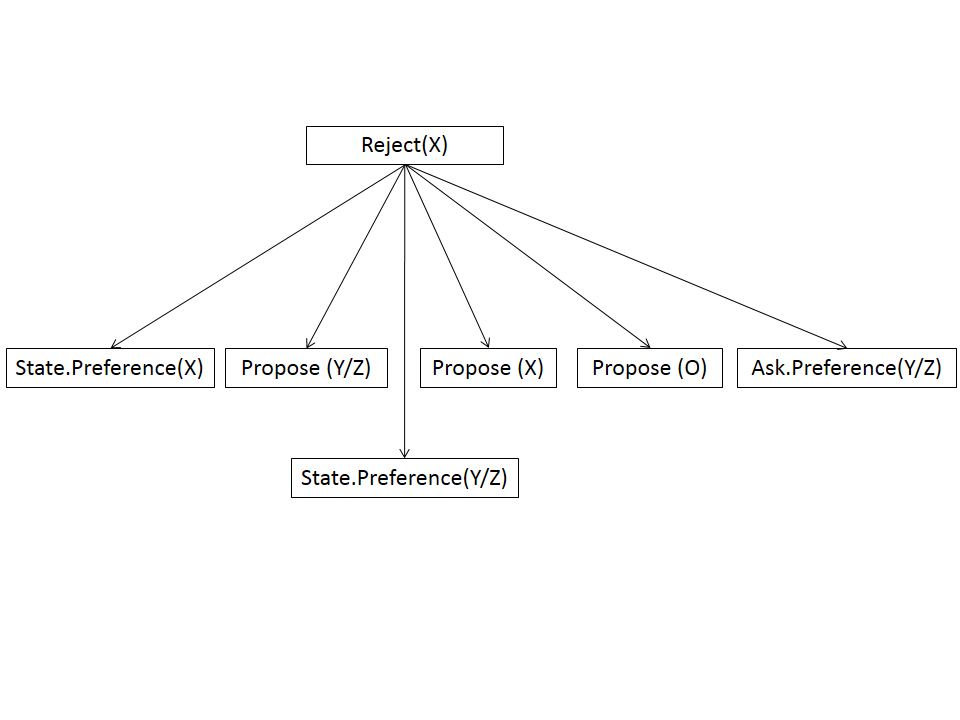
\includegraphics[width=5in]{figs/rejectX.PNG}}
%\vskip 8pt
%\defig{rejX}{agent possible answers to reject a value}
%\end{figure}
%
%\begin{enumerate}
% 
%\item propose($O$): the agent can  propose an option where $v(O,C)  \not= x$. For example
%\\ - User: Reject(italian): No, I'd raher choose something else.
%\\ -Agent: propose(chez chuck): Let's choose chez chuck!
%
%\item propose(x): As  explained before the agent can  propose  again the same value because he's very dominant, but we have to avoid a loop.
%
%\item Propose(y/z):the agent can also propose other values. 
%For example:
%\\ - User: Reject(cheeseClub). where (v(cheeseClub, cuisine) = fromage)
%\\ - agent: Propose (italian). 
%
%\item State.Preference(x): We can assume that the agent really like $x$ and in order to report to the user, he express his preference. Or in the contrary, to support the user reject, he can state that he doesn't like $x$ either. 
%Example: 
%\\ user: Reject(Italian): I'd rather choose something else.
%\\ Agent: State.Preference(Italian, *): I like the most italian
%\\ OR
%\\ agent: State.Preference(*, Italian): I like the least italian
%
%\item State.Preference($z$/$y$): the agent can state its preferences on other values for the different criteria. For example
%\\ User: Reject(italian)
%\\ agent:  State.Preference(French, *): I like the most french cuisine.
%
%\item   Ask.Preference($z$/$y$): the agent can also ask for the user preferences in order to make the right proposal next time.
%\\ User: Reject(italian)
%\\ agent:  Ask(French, *): Do you like french cuisine?
%
%\end{enumerate}
\end{document}